\documentclass[14pt]{extbook}
\usepackage{multicol, enumerate, enumitem, hyperref, color, soul, setspace, parskip, fancyhdr} %General Packages
\usepackage{amssymb, amsthm, amsmath, latexsym, units, mathtools} %Math Packages
\everymath{\displaystyle} %All math in Display Style
% Packages with additional options
\usepackage[headsep=0.5cm,headheight=12pt, left=1 in,right= 1 in,top= 1 in,bottom= 1 in]{geometry}
\usepackage[usenames,dvipsnames]{xcolor}
\usepackage{dashrule}  % Package to use the command below to create lines between items
\newcommand{\litem}[1]{\item#1\hspace*{-1cm}\rule{\textwidth}{0.4pt}}
\pagestyle{fancy}
\lhead{Makeup Progress Quiz 2}
\chead{}
\rhead{Version C}
\lfoot{2790-1423}
\cfoot{}
\rfoot{Summer C 2021}
\begin{document}

\begin{enumerate}
\litem{
Graph the equation below.\[ f(x) = -(x-1)^2 + 11 \]\begin{enumerate}[label=\Alph*.]
\begin{multicols}{2}\item 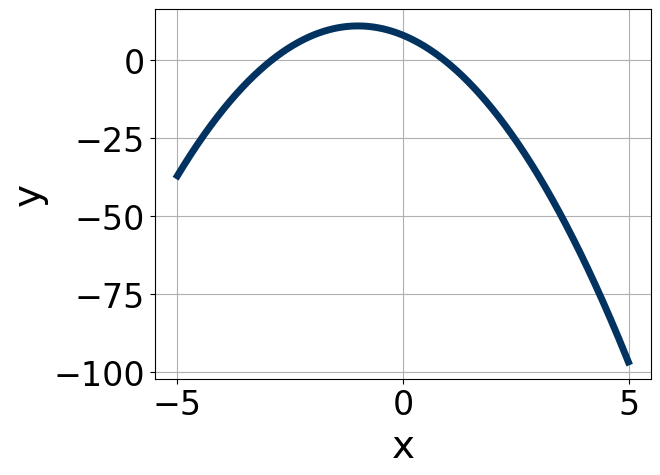
\includegraphics[width = 0.3\textwidth]{../Figures/quadraticEquationToGraphCopyAC.png}\item 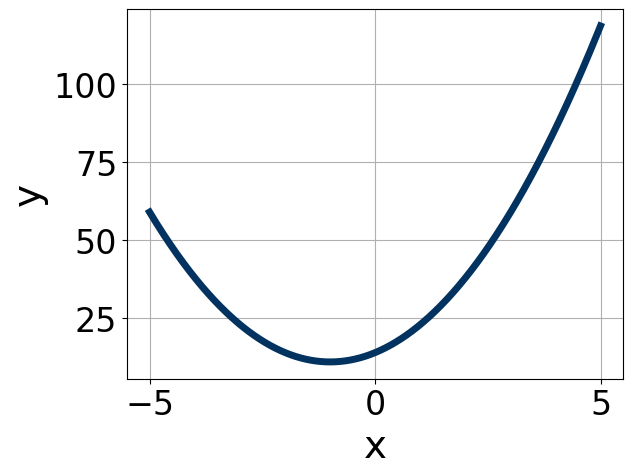
\includegraphics[width = 0.3\textwidth]{../Figures/quadraticEquationToGraphCopyBC.png}\item 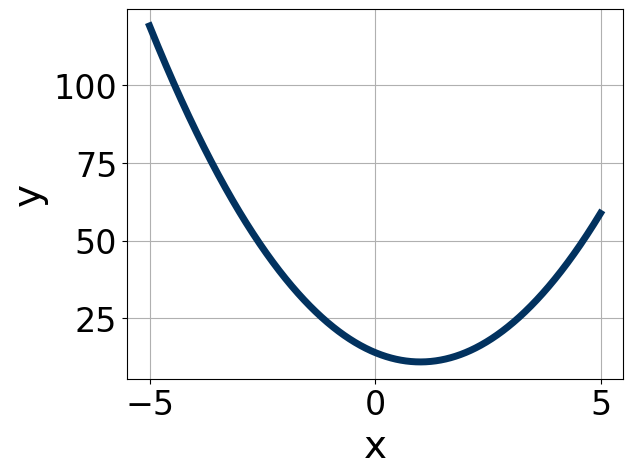
\includegraphics[width = 0.3\textwidth]{../Figures/quadraticEquationToGraphCopyCC.png}\item 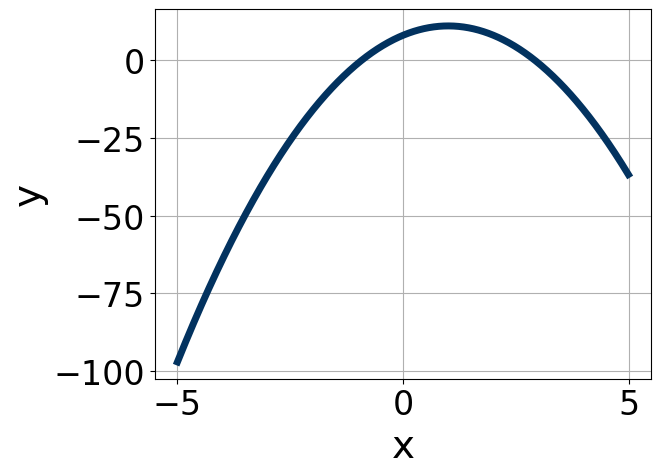
\includegraphics[width = 0.3\textwidth]{../Figures/quadraticEquationToGraphCopyDC.png}\end{multicols}\item None of the above.
\end{enumerate} }
\litem{
Solve the quadratic equation below. Then, choose the intervals that the solutions belong to, with $x_1 \leq x_2$ (if they exist).\[ 10x^{2} -13 x + 2 = 0 \]\begin{enumerate}[label=\Alph*.]
\item \( x_1 \in [-1.4, -0.1] \text{ and } x_2 \in [-0.18, 0.82] \)
\item \( x_1 \in [1.4, 2.4] \text{ and } x_2 \in [10.22, 12.22] \)
\item \( x_1 \in [-1.1, 1.2] \text{ and } x_2 \in [1.12, 6.12] \)
\item \( x_1 \in [-9, -8.5] \text{ and } x_2 \in [8.08, 11.08] \)
\item \( \text{There are no Real solutions.} \)

\end{enumerate} }
\litem{
Factor the quadratic below. Then, choose the intervals that contain the constants in the form $(ax+b)(cx+d); b \leq d.$\[ 81x^{2} +90 x + 25 \]\begin{enumerate}[label=\Alph*.]
\item \( a \in [-6, 2], \hspace*{5mm} b \in [41, 49], \hspace*{5mm} c \in [-0.4, 2.6], \text{ and } \hspace*{5mm} d \in [41, 52] \)
\item \( a \in [9, 10], \hspace*{5mm} b \in [5, 9], \hspace*{5mm} c \in [6.2, 12.3], \text{ and } \hspace*{5mm} d \in [0, 10] \)
\item \( a \in [22, 29], \hspace*{5mm} b \in [5, 9], \hspace*{5mm} c \in [1.7, 5], \text{ and } \hspace*{5mm} d \in [0, 10] \)
\item \( a \in [3, 7], \hspace*{5mm} b \in [5, 9], \hspace*{5mm} c \in [26.6, 27.5], \text{ and } \hspace*{5mm} d \in [0, 10] \)
\item \( \text{None of the above.} \)

\end{enumerate} }
\litem{
Solve the quadratic equation below. Then, choose the intervals that the solutions $x_1$ and $x_2$ belong to, with $x_1 \leq x_2$.\[ 25x^{2} +25 x -36 = 0 \]\begin{enumerate}[label=\Alph*.]
\item \( x_1 \in [-0.71, -0.32] \text{ and } x_2 \in [2.39, 2.41] \)
\item \( x_1 \in [-45.74, -44.28] \text{ and } x_2 \in [19.97, 20.18] \)
\item \( x_1 \in [-9.57, -7.92] \text{ and } x_2 \in [0.04, 0.25] \)
\item \( x_1 \in [-2.53, -1.43] \text{ and } x_2 \in [0.75, 0.81] \)
\item \( x_1 \in [-4.18, -3.5] \text{ and } x_2 \in [0.26, 0.64] \)

\end{enumerate} }
\litem{
Solve the quadratic equation below. Then, choose the intervals that the solutions belong to, with $x_1 \leq x_2$ (if they exist).\[ 11x^{2} -12 x + 3 = 0 \]\begin{enumerate}[label=\Alph*.]
\item \( x_1 \in [0.31, 0.51] \text{ and } x_2 \in [0.1, 0.8] \)
\item \( x_1 \in [3.88, 4.32] \text{ and } x_2 \in [6.8, 8] \)
\item \( x_1 \in [-3.3, -2.62] \text{ and } x_2 \in [2.1, 4.3] \)
\item \( x_1 \in [-1.63, 0.2] \text{ and } x_2 \in [-0.9, 0.2] \)
\item \( \text{There are no Real solutions.} \)

\end{enumerate} }
\litem{
Graph the equation below.\[ f(x) = -(x+1)^2 + 20 \]\begin{enumerate}[label=\Alph*.]
\begin{multicols}{2}\item 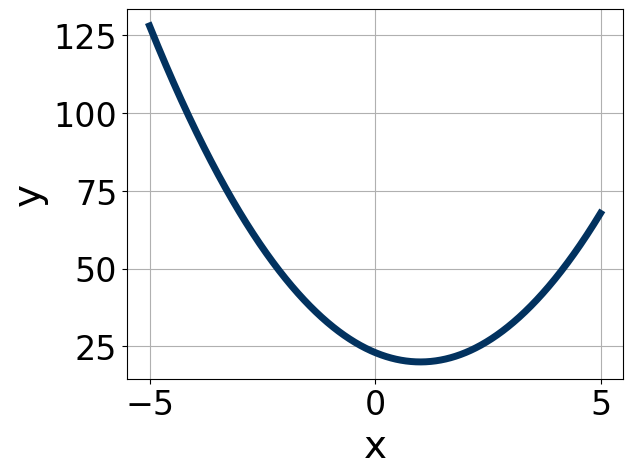
\includegraphics[width = 0.3\textwidth]{../Figures/quadraticEquationToGraphAC.png}\item 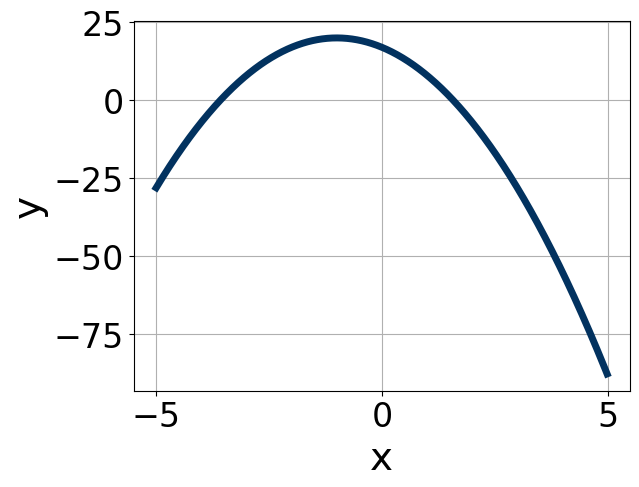
\includegraphics[width = 0.3\textwidth]{../Figures/quadraticEquationToGraphBC.png}\item 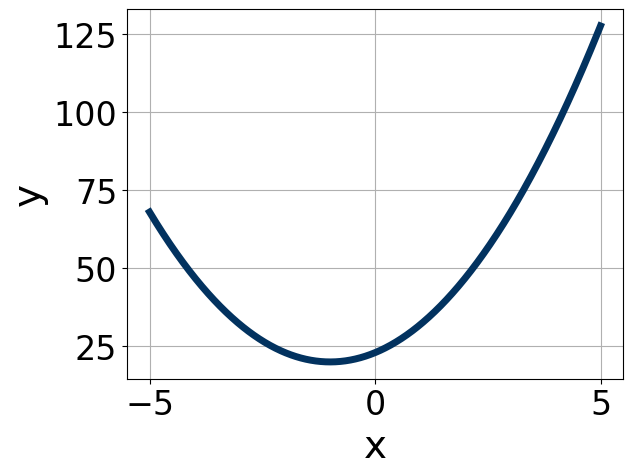
\includegraphics[width = 0.3\textwidth]{../Figures/quadraticEquationToGraphCC.png}\item 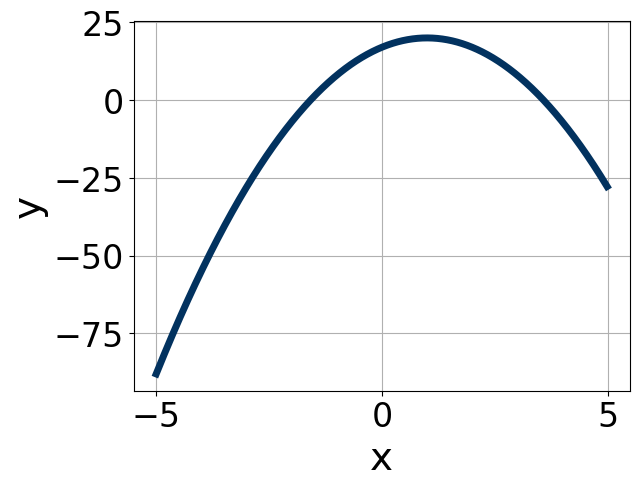
\includegraphics[width = 0.3\textwidth]{../Figures/quadraticEquationToGraphDC.png}\end{multicols}\item None of the above.
\end{enumerate} }
\litem{
Solve the quadratic equation below. Then, choose the intervals that the solutions $x_1$ and $x_2$ belong to, with $x_1 \leq x_2$.\[ 25x^{2} -50 x + 24 = 0 \]\begin{enumerate}[label=\Alph*.]
\item \( x_1 \in [0.18, 0.28] \text{ and } x_2 \in [3.53, 4.07] \)
\item \( x_1 \in [0.62, 0.83] \text{ and } x_2 \in [0.84, 1.28] \)
\item \( x_1 \in [19.98, 20.03] \text{ and } x_2 \in [29.73, 30.11] \)
\item \( x_1 \in [0.55, 0.73] \text{ and } x_2 \in [1.47, 2.23] \)
\item \( x_1 \in [0.33, 0.55] \text{ and } x_2 \in [1.9, 2.69] \)

\end{enumerate} }
\litem{
Write the equation of the graph presented below in the form $f(x)=ax^2+bx+c$, assuming  $a=1$ or $a=-1$. Then, choose the intervals that $a, b,$ and $c$ belong to.
\begin{center}
    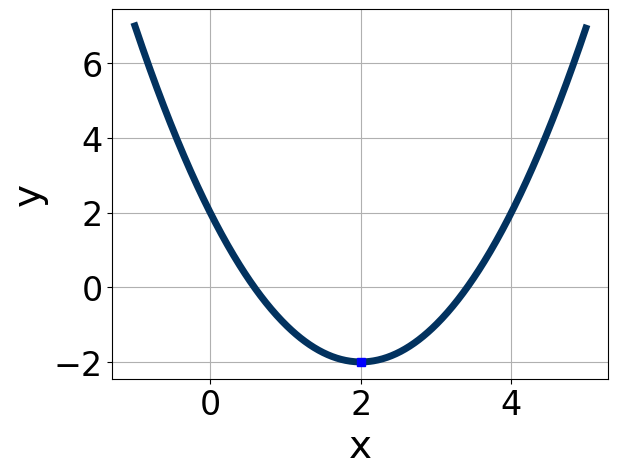
\includegraphics[width=0.5\textwidth]{../Figures/quadraticGraphToEquationC.png}
\end{center}
\begin{enumerate}[label=\Alph*.]
\item \( a \in [-1, 0], \hspace*{5mm} b \in [4, 7], \text{ and } \hspace*{5mm} c \in [-7, -4] \)
\item \( a \in [0, 5], \hspace*{5mm} b \in [4, 7], \text{ and } \hspace*{5mm} c \in [0, 4] \)
\item \( a \in [0, 5], \hspace*{5mm} b \in [4, 7], \text{ and } \hspace*{5mm} c \in [4, 8] \)
\item \( a \in [0, 5], \hspace*{5mm} b \in [-4, -3], \text{ and } \hspace*{5mm} c \in [0, 4] \)
\item \( a \in [-1, 0], \hspace*{5mm} b \in [-4, -3], \text{ and } \hspace*{5mm} c \in [-7, -4] \)

\end{enumerate} }
\litem{
Factor the quadratic below. Then, choose the intervals that contain the constants in the form $(ax+b)(cx+d); b \leq d.$\[ 54x^{2} -69 x + 20 \]\begin{enumerate}[label=\Alph*.]
\item \( a \in [5.94, 7.72], \hspace*{5mm} b \in [-5, -3], \hspace*{5mm} c \in [5, 13], \text{ and } \hspace*{5mm} d \in [-6, -3] \)
\item \( a \in [0.23, 1.4], \hspace*{5mm} b \in [-49, -43], \hspace*{5mm} c \in [1, 3], \text{ and } \hspace*{5mm} d \in [-24, -23] \)
\item \( a \in [1.09, 2.11], \hspace*{5mm} b \in [-5, -3], \hspace*{5mm} c \in [27, 28], \text{ and } \hspace*{5mm} d \in [-6, -3] \)
\item \( a \in [11.78, 12.62], \hspace*{5mm} b \in [-5, -3], \hspace*{5mm} c \in [3, 6], \text{ and } \hspace*{5mm} d \in [-6, -3] \)
\item \( \text{None of the above.} \)

\end{enumerate} }
\litem{
Write the equation of the graph presented below in the form $f(x)=ax^2+bx+c$, assuming  $a=1$ or $a=-1$. Then, choose the intervals that $a, b,$ and $c$ belong to.
\begin{center}
    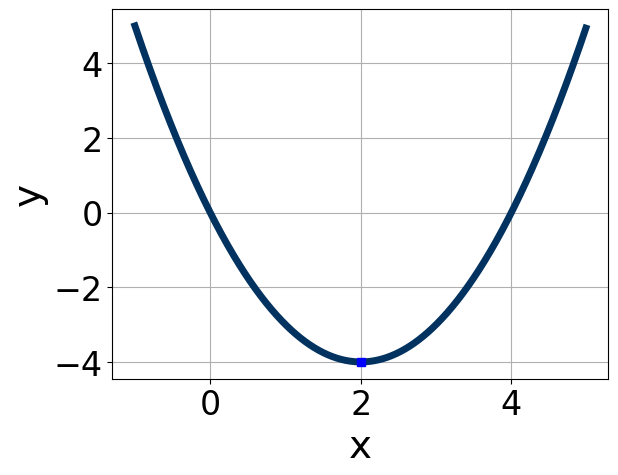
\includegraphics[width=0.5\textwidth]{../Figures/quadraticGraphToEquationCopyC.png}
\end{center}
\begin{enumerate}[label=\Alph*.]
\item \( a \in [0.5, 2.3], \hspace*{5mm} b \in [2, 6], \text{ and } \hspace*{5mm} c \in [-1, 1] \)
\item \( a \in [-1.2, 0.5], \hspace*{5mm} b \in [2, 6], \text{ and } \hspace*{5mm} c \in [-8, -5] \)
\item \( a \in [-1.2, 0.5], \hspace*{5mm} b \in [-7, 0], \text{ and } \hspace*{5mm} c \in [-8, -5] \)
\item \( a \in [0.5, 2.3], \hspace*{5mm} b \in [-7, 0], \text{ and } \hspace*{5mm} c \in [-1, 1] \)
\item \( a \in [0.5, 2.3], \hspace*{5mm} b \in [2, 6], \text{ and } \hspace*{5mm} c \in [8, 10] \)

\end{enumerate} }
\end{enumerate}

\end{document}